\begin{itemize}
	\item While climate science research has focused on predicted climate effects of SRM, \textbf{few studies have investigated impacts that SRM would have on ecological systems}.
	\item Impacts and risks posed by SRM would vary by implementation scenario, anthropogenic climate effects, geographic region, and by ecosystem, community, population, and organism.

\end{itemize}

\begin{figure}
	\begin{center}
		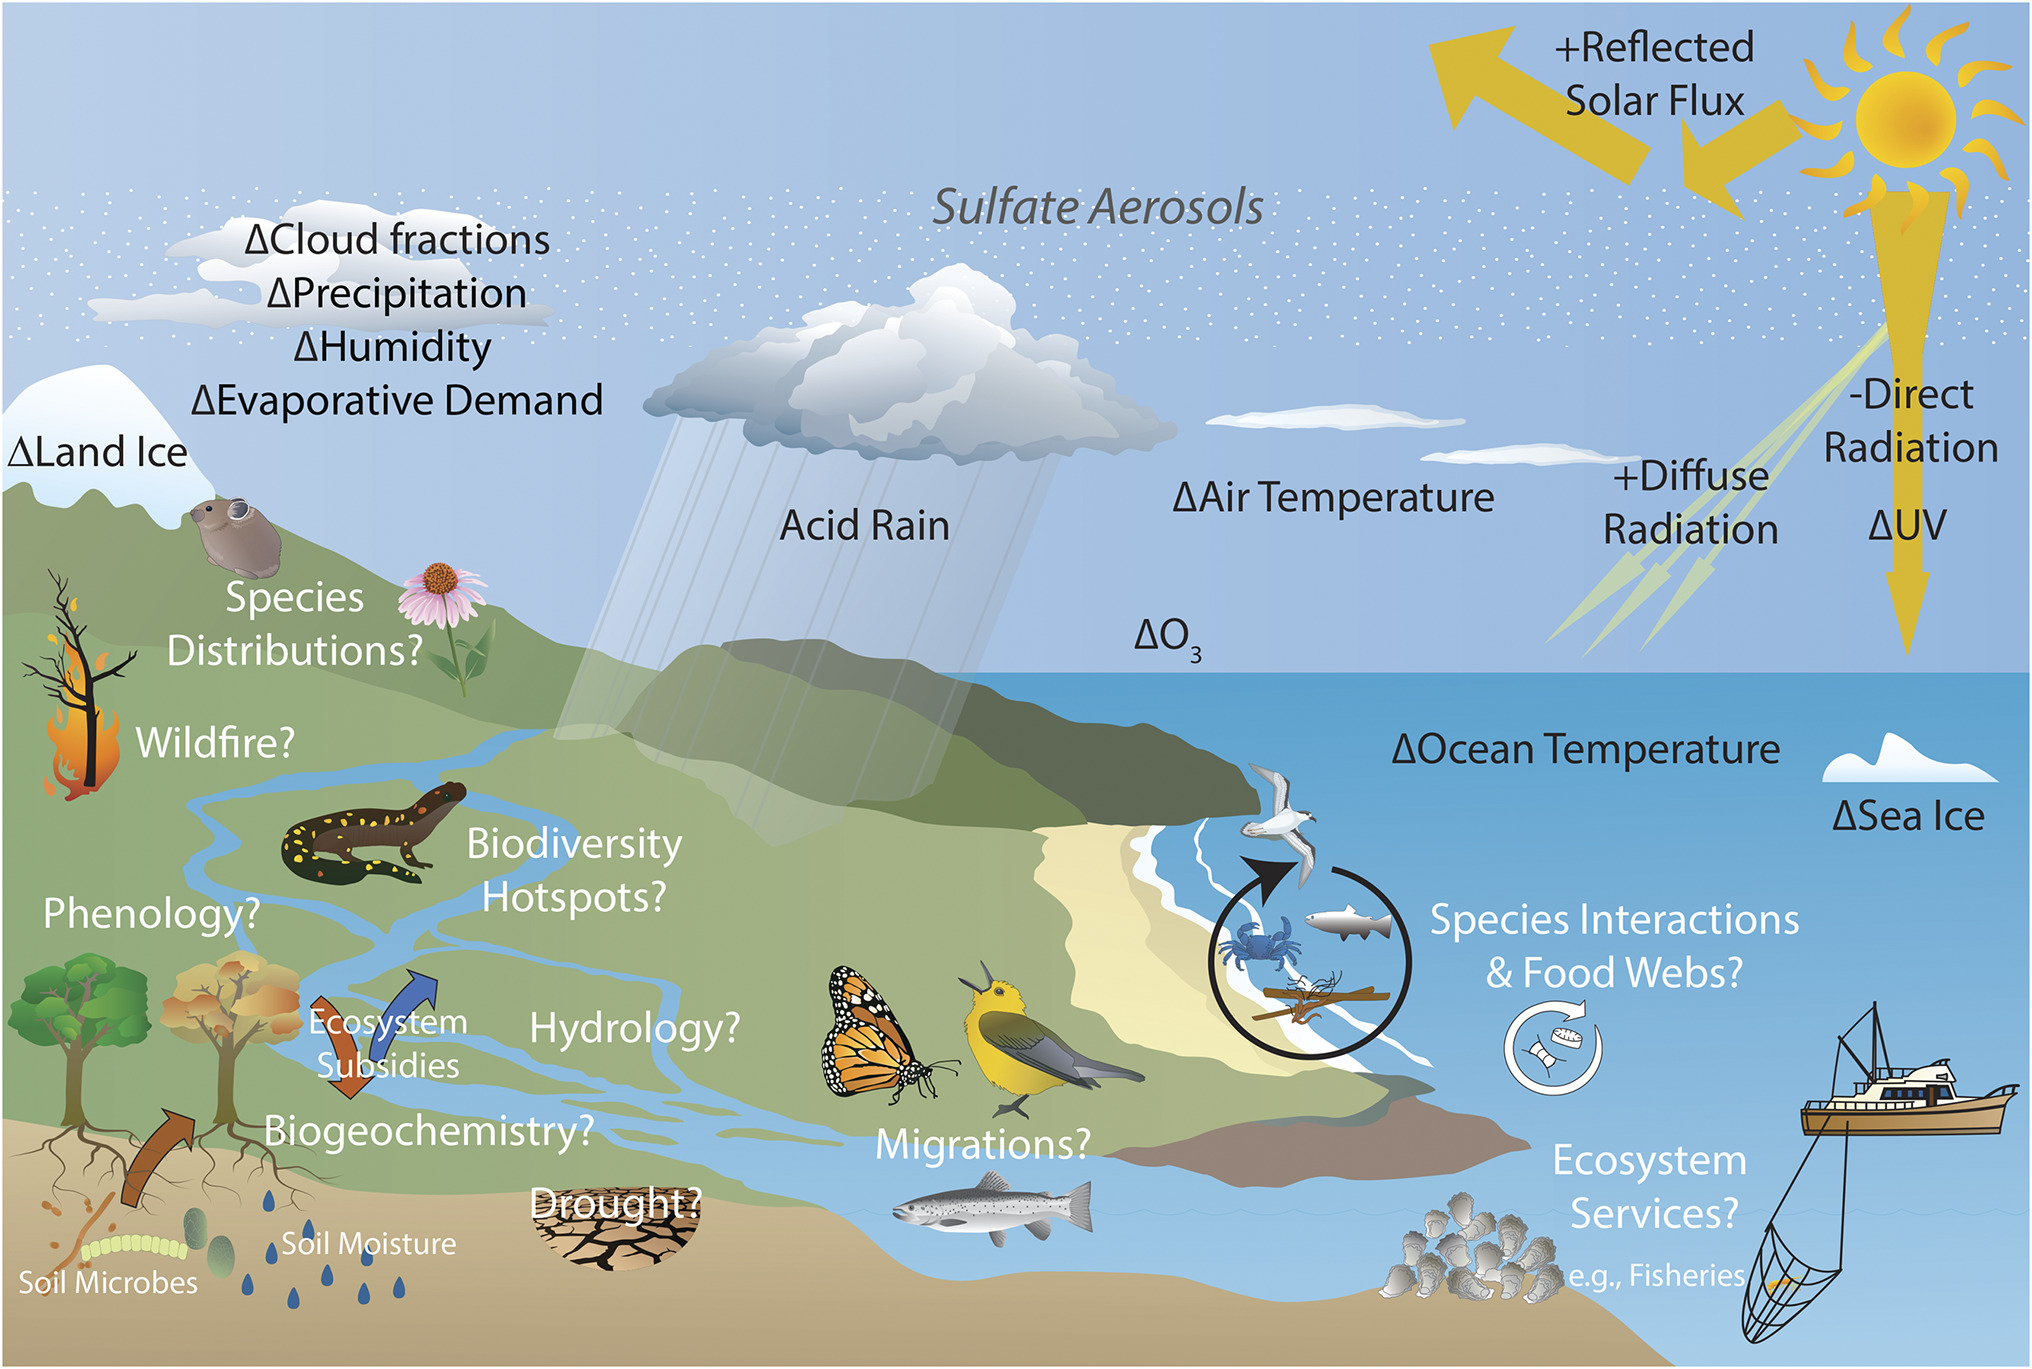
\includegraphics[width=0.8\columnwidth]{figures/pnas.1921854118fig01.jpg}
	\end{center}
	\caption{Although some effects of SRM with SAI on the climate are known from certain SAI scenarios (indicated with $+$ for likely increases, $-$ for decreases, $\Delta$ to indicate change), the effects of SAI on ecological systems are largely unknown. Adopted from Zarnetske et al. (2021).
		% https://www.pnas.org/doi/10.1073/pnas.1921854118
	}
\end{figure}

\begin{itemize}
	\item Models used for projecting responses to SAI are often the same Earth system models (ESMs) used to study anthropogenic climate change effects without SAI.
	\item These models must additionally be able to represent complex stratospheric aerosol processes and ecological responses and feedbacks.

	\item \textbf{A transdisciplinary approach, increasing collaboration between ecologists and climate scientists, is essential} for understanding the benefits and risks of SAI on climate and to ecological systems.
\end{itemize}

